\documentclass[../algorithms.tex]{subfiles}
\begin{document}
In this chapter, we talk about recursive function and how to write a recursive function that work properly. Then we give an algorithm theory: divide and conquer, which is a recursive function and divide problems, and solve problems separely, the final result is merged from the result of each subproblem. Also we need to understand the space and time complexity. 
%%%%%%%%%%%%%%%%%%%%%%%%%%%%%%%%%%%%%%%%%%%%%%%%%%%%%%%%%%%%%%%%%%%%%%%%%%%%%%%%%%%%%
%%%%%%%%%%%%% Recursive Programming
%%%%%%%%%%%%%%%%%%%%%%%%%%%%%%%%%%%%%%%%%%%%%%%%%%%%%%%%%%%%%%%%%%%%%%%%%%%%%%%%%%%%%%%%%
\section{Recursive Programming}
For recursive function, we can draw recursive tree to denote the state transfer graph. With recursive function, it can simplify the programming of certain programs, once we mastered recursive function, we would feel it is a lot simpler than iterative implementation. However, it does take extra space complexity compared with the iterative implementation. 

\textbf{Recursive Function}: for recusrive program, we need to figure out the recursive transfer function between $f(i)$ and the next level $f(i+1)$. For example, the fibonacci number we could have $f(i) = f(i-1) + f(i-2)$. For the merge sort, we cant use a math function to represent this operation, we have $T(n) = 2*T(n/2) + O(n)$. $f(i) = merge(f(left), f(right))$. Some recursive function would have redundancy which we can improve the efficiency and avoid to compute the same subproblem twice by memoization which saves the result, and the iterative peer of the recursive implementation is called \textit{dynamic programming}. We will discuss the dynamic programming in details in the following chapter ~\ref{dynamic-programming}. Some other recursive function, there is no overlaps between subproblems which are the \textit{divide and conquer} cases, which will be discussed in detain in chapter~\ref{divide-conquer}. Or we have the universal \textit{Depth-first-searching} which can be implemented with recursive function, we will include this in chapter~\ref{searching}. 

\textbf{Recursive Function and Tree Structure}: 

\textbf{Stack Overflow and Iterative Implementation}: According to Wikepedia, in software, a stack overflow occurs if the call stack pointer exceeds the stack bound. The call stack may consist of a limited amount of address space, often determined at the start of the program depending on many factors, including the programming language, machine architecture, multi-threading, and amount of available memory. When a program attemps to use more space than is available on the call stack, the stack is said to \textit{overflow}, typically resulting in a program crash. The very deep recursive function is faced with the threat of stack overflow. And the only way we can fix it is by transforming the recursion into a loop and storing the function arguments in an explicit stack data structure, this is often called the iterative implementation which corresponds to the recursive implementation. 

We need to follow these points:
\begin{enumerate}
    \item End condition, Base Cases and Return Values: either return an answer for base cases or None, and used to end the recursive calls.  
    \item Parameters: parameters include: data needed to implement the function, current paths, the global answers and so on. 
    \item Variables: What the \textbf{local} and {global} variables. In Python any pointer type of data can be used as global variable global result putting in the parameters. 
    \item Construct current result: when to collect the results from subtree and combine to get the result for current node.
    \item Check the depth: if the program will lead to the heap stack overflow.
\end{enumerate}


% 递归函数关注以下几个因素
% ·退出条件
% ·参数有哪些
% ·返回值是什么
% ·局部变量有哪些
% ·全局变量有哪些
% ·何时输出
% ·会不会导致堆栈溢出
%%%%%%%%%%%%%%%%%%%%%%%%%%%%%%%%%%%%%%%%%%%%%%%%%%%%%%%%%%%%%%%%%%%%%%%%%%%%%%%%%%%%%
%%%%%%%%%%%%% Divide and Conquer
%%%%%%%%%%%%%%%%%%%%%%%%%%%%%%%%%%%%%%%%%%%%%%%%%%%%%%%%%%%%%%%%%%%%%%%%%%%%%%%%%%%%%%%%%
\section{Divide and Conquer}
Divide and conquer partitions the problems into smaller subproblems and solves the problems recursively, and then combine the solutions to solve the original problem. It includes three steps at each recursive call:
\begin{enumerate}
    \item Divide: divide one problems into a series of subproblems that are smaller instances of the same problem;
    \item Conquer: recursively solve each subproblem. When the subproblem is small enough, it will be solved directly, which is the end condition in the recursive function; 
    \item Combine: combine the result from each subproblem into the solution to the current problem.
\end{enumerate}

For divide and conquer, we have two cases, 1) our subproblems are disjoint with each other; 2) our smaller subproblem can include another smaller subproblem. We can use the the following two recurrence equation to generalize.
\begin{equation} \label{bt_time}
\begin{split}
T(n) & = aT(n/b) + f(n)\\
\end{split}
\end{equation}
where $f(n)$ denotes the time and operation need to divide the problem into disjoint and independent subproblems and combine the solutions of the subproblems to solve the current problem. 
\begin{equation} \label{dp_equation}
\begin{split}
T(n) &= T(n-1) + T(n-2) +...+T(1) + f(n)\\
\end{split}
\end{equation} 
 We can have any combination of terms $T(k), k = [1, n-1]$ on the right side of this recurrence equation. Here the problem is divided into subproblems, however these problem are not disjoint and always depend on other. And the subproblems overlap, which is to say, when subproblems share subproblems. 
 
 Because of the different relations between these two situations' subproblems, Eq.~\ref{bt_time} when we use recursive programming to solve the problem directly, we get the best time complexity since there is no overlap between subproblems. However, for the second case in Eq.~\ref{dp_equation}, programming them recursivly would end up with redundancy in time complexity becase their subproblems share subproblems. This also means they can be further optimized, and these type of algorithms fall in the category of dynamic programming which we will discuss in the next chapter in details. So, commonly divide and conquer refers to methods in the first category. 
 
 Now, enough of the concepts, let us look at an example:
 
 Example 1: Maximum Subarray (53. medium)
\begin{lstlisting}

Find the contiguous subarray within an array (containing at least one number) which has the largest sum.

For example, given the array [-2,1,-3,4,-1,2,1,-5,4],
 the contiguous subarray [4,-1,2,1] has the largest sum = 6.
\end{lstlisting}
divide and conquer solution: $T(n) = max(T(left),T(right), T(cross))$, max is for merging and the T(cross) is for the case that the potential subarray across the mid point. For the complexity, $T(n)=2T(n/2)+n$, if we use the master method, it would give us $O(nlgn)$. We write the following Python code
\begin{lstlisting}[language = Python]
def maxSubArray(self, nums):
        """
        :type nums: List[int]
        :rtype: int
        """
        def getCrossMax(low,mid,high):
            left_sum,right_sum =0,0
            left_max,  right_max = -maxint, -maxint
            left_i,right_j=-1,-1
            for i in xrange(mid,low-1,-1): #[)
                left_sum+=nums[i]
                if left_sum>left_max:
                    left_max= left_sum
                    left_i = i
            for j in xrange(mid+1,high+1):
                right_sum+=nums[j]
                if right_sum>right_max:
                    right_max= right_sum
                    right_j = j
            return (left_i,right_j,left_max+right_max)
        
        def maxSubarray(low,high):
            if low==high:
                return (low,high, nums[low])
            mid = (low+high)//2
            rslt=[]
            #left_low, left_high, left_sum = maxSubarray(low,mid) #[low,mid]
            rslt.append(maxSubarray(low,mid)) #[low,mid]
            #right_low,right_high,right_sum = maxSubarray(mid+1,high)#[mid+1,high]
            rslt.append(maxSubarray(mid+1,high))
            #cross_low,cross_high,cross_sum = getCrossMax(low, mid, high)
            rslt.append(getCrossMax(low, mid, high))
            return max(rslt, key=lambda x: x[2])
        return maxSubarray(0,len(nums)-1)[2]
\end{lstlisting}
Also, we does not necessarily to use divide and conquer, we can be more creative and try harder to make the time complexity goes to $O(n)$. We can convert this problem to best time to buy and sell stock problem.[0, -2, -1, -4, 0, -1, 1, 2, -3, 1], => O(n), then we use prefix\_sum, the difference is we set prefix\_sum to 0 when it is smaller than 0, O(n)
\begin{lstlisting}[language = Python]
from   sys import maxint
class Solution(object):    
    def maxSubArray(self, nums):
        """
        :type nums: List[int]
        :rtype: int
        """
        max_so_far = -maxint - 1
        prefix_sum= 0
        for i in range(0, len(nums)):
            prefix_sum+= nums[i]
            if (max_so_far < prefix_sum):
                max_so_far = prefix_sum
 
            if prefix_sum< 0:
                prefix_sum= 0  
        return max_so_far
\end{lstlisting}
%%%%%%%%%%%%%%%%%%%%%%%%%%%%%%%%%%%%%%%%%%%%%%%%%%%%%%%%%%%%%%%%%%%%%%%%%%%%%%%%%%%%%
%%%%%%%%%%%%% Complexity Analysis
%%%%%%%%%%%%%%%%%%%%%%%%%%%%%%%%%%%%%%%%%%%%%%%%%%%%%%%%%%%%%%%%%%%%%%%%%%%%%%%%%%%%%%%%%
\section{Complexity Analysis}
The complexity analysis incldudes the time and space complexity. While for the divide and conquer methods, because of the usage of the recursion function, it could be slightly tricky and we need to learn how to attack this complexity. Also it is usually required and asked by interviewers in real interview.

\subsection{Time Complexity}
The core to analyze the time complexity of the divide and conquer methodology is by characterizing the recurrence relation shown in Eq.~\ref{bt_time}. In general we have three ways to do this, 1) substitution method; 2) recursion-tree method; 3) master method. However, in real situation, it depends on XX to choose which one to use. Each one has its own limitation. In this book, we prove enough theory about how to compute the time complexity for the recurrence equation for practical coding or interview situation. If you want to learn more, it is a good choice to refer the book (Introduction to Algorithms). Here, we wont detail on the substitution method, because in real interviews, we need some quick and more straightforward ways to get the computational cost. And the substitution method is more used to prove the cost in a very rigorous way. Recursion tree and the master therorems are the main ways we rely on to answer the time complexity for a divide and conquer method shown in Eq.~\ref{bt_time}. 

\subsubsection{Recursion Tree Method}
Drawing out a recursion tree serves as a straightforward way to come up with a good guess. Normally we can tolerate a small amount of "sloppiness", because later on, we can prove the complexity with substitution method discussed in the last section. However, when we are drawing the recursion tree, if we are careful enough and summing up the costs from each level and each node, we can use is as a direct proof of the solution to the recurrence. 

In the corresponding recursion tree for recurrence equation in divide and conquer, each node represents the cost of a single subproblem somewhere in the set of recursive function invocations. We sum the costs within each level of the tree to obtain a set of per-level costs, and then we sum all the per-level costs to determine the total cost of all levels of the recursion. Let's look at one example for given recursion $T(n) = 3T(\floor*{n/4}) + \Theta(n^2)$. We replace $\Theta(n^2) = cn^2$, where $c>0$. $cn^2$ is the cost we pay to divide a problem with $n$ input size to three problems each with $n/4$ input size and combine the solution of the subproblems to solve the current problem.  We first expand $T(n)$, and put the cost $cn^2$ at the root, and with three children each noted with $T(n/4)$. Then we recursively replace $T(n/4)$ with the cost and its subproblem till the size of each subproblem to be 1, which means we get to the leaves. The computational complexity for this recursion would be the sum of all layers's costs. And we assume $T(1)=1$.
\begin{figure}[h]
    \centering
    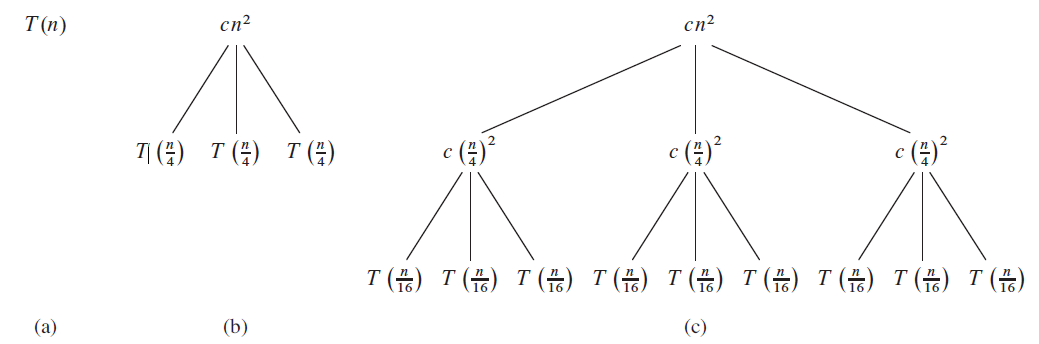
\includegraphics[width=0.8\columnwidth]{fig/recursive_tree_1.png}
    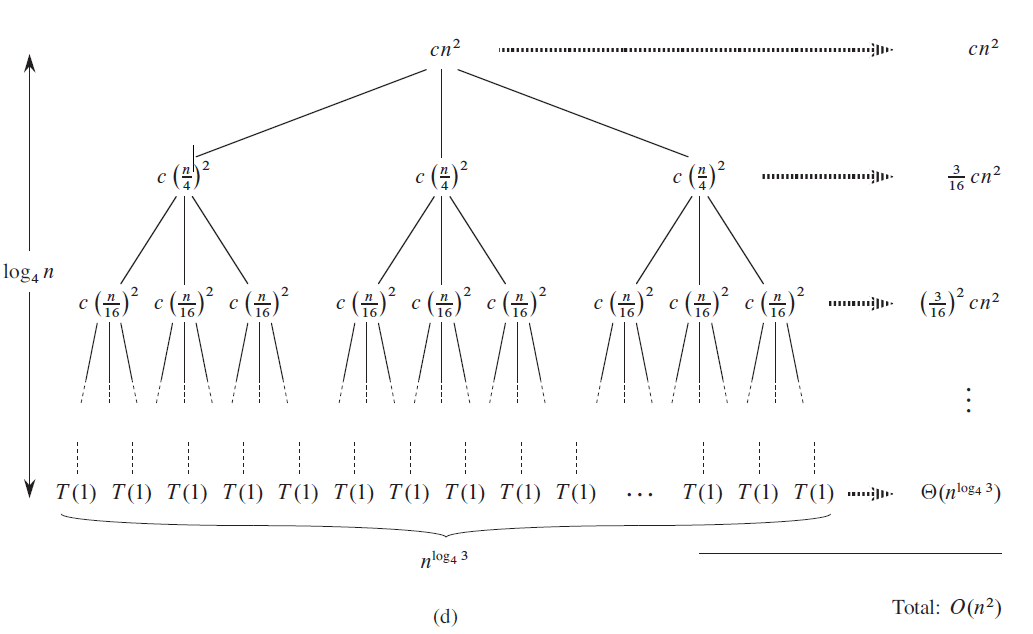
\includegraphics[width=0.8\columnwidth]{fig/recursive_tree_2.png}
    \caption{The process to construct a recursive tree for $T(n) = 3T(\floor*{n/4}) + cn^2$}
    \label{fig:recursive_tree}
\end{figure}
\begin{equation} \label{eg_recurrence_5}
\begin{split}
T(n) & = cn^2+\frac{3}{16}cn^2+(\frac{3}{16})^2cn^2+...+(\frac{3}{16})^{\log_4 {n-1}}cn^2+\Theta(n^{\log_4 3})\\
& = \sum_{i=0}^{\log_4 {n-1}}(\frac{3}{16})^{i}cn^2+\Theta(n^{\log_4 3})\\
&< \sum_{i=0}^{\infty}(\frac{3}{16})^{i}cn^2+\Theta(n^{\log_4 3})\\
& = \frac{1}{1-(3/16)} cn^2+\Theta(n^{\log_4 3})\\
& = O(n^2).
\end{split}
\end{equation}
\subsubsection{Master Method}
The master method is probably the easiest way to come up with the computational complexity analysis. It is a theorem that are proved by researchers, and we just need to learn how to use them. The master theorem goes:

For Eq.~\ref{bt_time}, let $a\geq1, b>1$, we first compute $n^{\log_b a}$, 
\begin{enumerate}
    \item If $f(n) = O(n^{\log_b a - \epsilon}$ for constant $\epsilon>0$, then we get $T(n) = \Theta(n^{\log_b a})$.
    \item If $f(n) = \Theta(n^{\log_b a }$, then we get $T(n) = \Theta(n^{\log_b a} \log n)$.
    \item If $f(n) = \Omega(n^{\log_b a + \epsilon}$ for constant $\epsilon>0$, and if $a f(n/b)\leq cf(n)$ for constant $c<1$ and all sufficiently large $n$, then we get $T(n) = \Theta(f(n))$.
\end{enumerate}
\subsection{Space Complexity}
The space the recursive function occupies is rational to the depth of the recursive calls, $O(h)$, $h$ is the height of the recursive tree.

\subsection{Summary}
For your convenience, we prove a table that shows the frequent used recurrence equations' time complexity. 
\begin{figure}[h]
    \centering
    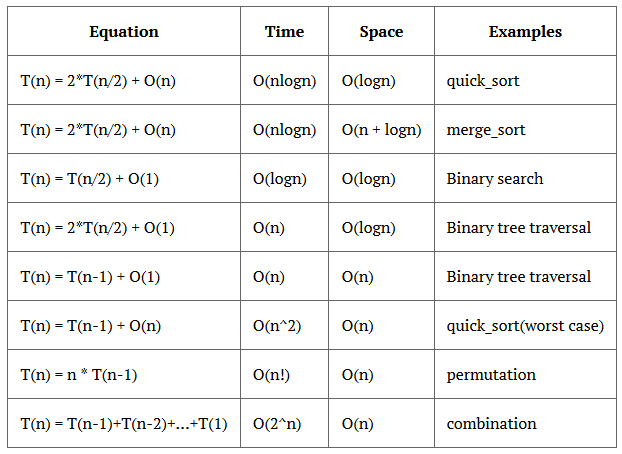
\includegraphics[width=1\columnwidth] {fig/complexity_cheatsheet.png}
    \caption{The cheat sheet for time and space complexity with recurrence function.}
    \label{fig:cheat_sheet}
\end{figure}
%%%%%%%%%%%%%%%%%%%%%%%%%%%%%%%%%%%%%%%%%%%%%%%%%%%%%%%%%%%%%%%%%%%%%%%%%%%%%%%%%%%%%
%%%%%%%%%%%%% Exercises
%%%%%%%%%%%%%%%%%%%%%%%%%%%%%%%%%%%%%%%%%%%%%%%%%%%%%%%%%%%%%%%%%%%%%%%%%%%%%%%%%%%%%%%%%
\section{Exercises}
\begin{enumerate}
    \item Pow(x, n) (50)
    
    Solution: T(n)= T(n/2)+O(1), the complexity is the same as the binary search, $O(logn)$.
    \begin{lstlisting}[language=Python]
    def myPow(self, x, n):
        """
        :type x: float
        :type n: int
        :rtype: float
        """
        if n==0:
            return 1
        if n<0:
            n=-n
            x=1.0/x
        def helper(n):
            if n==1:
                return x
            
            h = n//2
            r = n-h
            value = helper(h) #T(n/2), then we have O(1)
            if r==h:                
                return value*value
            else: #r is going to be 1 bigger
                return value*value*x
        return helper(n)
    \end{lstlisting}
    
    \item House Robber (198)
    
    Solution: If we use brute force is $O(2^n)$. Use divide and conquer, here because we use half and half. Which we need to get rid of. 
\begin{lstlisting}[language = Python]
def rob(self, nums):
        """
        :type nums: List[int]
        :rtype: int
        """
        memo=[[-1 for _ in range(len(nums))] for _ in range(len(nums))]
        
        def dp(l,r):
            nonlocal memo
            if l==r:
                return nums[l]
            if l>r:
                return 0
            if l<r:
                if memo[l][r]==-1:
                    mid=l+(r-l)//2
                    value = nums[mid] +dp(l,mid-2)+dp(mid+2,r)#take this value
                    not_value =dp(l,mid-1)+dp(mid+1,r) #not take
                    memo[l][r]=max(value, not_value)
                return memo[l][r]
        return dp(0,len(nums)-1)
\end{lstlisting}

\item Create Maximum Number (321) 

Given two arrays of length m and n with digits 0-9 representing two numbers. Create the maximum number of length k <= m + n from digits of the two. The relative order of the digits from the same array must be preserved. Return an array of the k digits. You should try to optimize your time and space complexity.
\begin{lstlisting}
Example 1:

nums1 = [3, 4, 6, 5]
 nums2 = [9, 1, 2, 5, 8, 3]
 k = 5
 return [9, 8, 6, 5, 3]

Example 2:

nums1 = [6, 7]
 nums2 = [6, 0, 4]
 k = 5
 return [6, 7, 6, 0, 4]

Example 3:

nums1 = [3, 9]
 nums2 = [8, 9]
 k = 3
 return [9, 8, 9]

\end{lstlisting}

Solution: First use DP + memo: LTE, 70/120 passed. We should use greedy and solve each array to find i,j, i+j = k, then we combine them.
\begin{lstlisting}[language=Python]
def maxNumber(self, nums1, nums2, k):
        """
        :type nums1: List[int]
        :type nums2: List[int]
        :type k: int
        :rtype: List[int]
        """
        '''i, j T(i,j,k)= max(nums[i]*10^k-1+T(i+1,j,k-1), j, T(i+1,j+1,k)), for the third iterm, the restriction is we need the left       elements>=k'''
        n1=len(nums1)
        n2=len(nums2)
        memo=[[[None for k in range(k+1)] for col in range(n2+1) ] for row in range(n1+1)]
        def dp(i,j,k):
            if k==0:
                return 0
            if memo[i][j][k] is None:
                max1,max2,max3=-1,-1,-1
                if i<len(nums1):
                    tmp =dp(i+1, j, k-1) #take i
                    tmp2 = dp(i+1,j,k) #neglect i in nums1
                    if tmp!=-1:
                        max1 = nums1[i]*(10**(k-1))+tmp
                    max1=max(max1,tmp2)
                if j<len(nums2):
                    tmp = dp(i, j+1, k-1) #take j
                    tmp2=dp(i,j+1,k) #neglect j in nums2
                    if tmp!=-1:
                        max2 = nums2[j]*(10**(k-1))+tmp
                    max2=max(max2,tmp2)
                memo[i][j][k] = max(max1,max2)
            return memo[i][j][k] 
        r = dp(0,0,k)
        rst=[]
        for i in range(k-1,-1,-1):
            rst.append(r//(10**i))
            r = r%(10**i)
            
        return rst
\end{lstlisting}

\item Best Time to Buy and Sell Stock (121)

Say you have an array for which the ith element is the price of a given stock on day i.

If you were only permitted to complete at most one transaction (ie, buy one and sell one share of the stock), design an algorithm to find the maximum profit.
\begin{lstlisting}[language=Python]
Example 1:

Input: [7, 1, 5, 3, 6, 4]
Output: 5

max. difference = 6-1 = 5 (not 7-1 = 6, as selling price needs to be larger than buying price)

Example 2:

Input: [7, 6, 4, 3, 1]
Output: 0

In this case, no transaction is done, i.e. max profit = 0.
\end{lstlisting}

Solution: Step 1: convert it to the maximum subarray problem. The first example is, [7–7=0,1–7=-6,5–1=4,3–5=-2,6–3=3, 4–6=-2],set the first element to 0, then the second is nums[i]-[nums[i-1], [0,-6,4,-2,3,-2] =>[0+6, 6–6=0, 0+4=4, 4–2=2, ] Set the first to 0+6, nums[i-1]+nums[i].

r = max(left\_subarray, right\_subarry, max(right\_subarry)-min(left\_subarray)), Thus, the real operation is max(right\_subarry)-min(left\_subarray). The time complexity would be decreased to $O(nlgn)$ from the brute force $O(n^2)$. So this example shows the divide and conquer. However, it might not be the best solution. Try the BCR with $O(n)$.
\begin{lstlisting}[language=Python]
class Solution(object):
    def maxProfit(self, prices):
        """
        :type prices: List[int]
        :rtype: int
        """
        if len(prices)<=1:
            return 0
    
        r = -maxint
        min_price = maxint
        for price in prices:
            if price<min_price:
                min_price = price
            else:
                r = max(r,price-min_price)
            
        return 0 if r<0 else r
\end{lstlisting}
\end{enumerate}
\end{document}